% paper/tex/experiment.tex
% Auto-refreshed by scripts/init_paper.py. Hand-edit the prose; placeholder
% tables and figures are wired via \input{} so re-running gen_latex_table.py
% refreshes them without touching this file.

\section{Experiments}\label{sec:experiments}

We test three claims. (C1) GRACE attains the highest \emph{goal
completeness} on the AI2-THOR household benchmark across three
open-weight LLMs. (C2) Each of GRACE's three components --- the
symbolic verifier, the local repair operator, and the hybrid memory
store --- contributes a distinct, measurable improvement. (C3)
GRACE's plans satisfy a \emph{strict} precondition check that
exposes baselines as silently invalid even when their heuristic
precondition score is~$1.0$.

\subsection{Setup}\label{sec:setup}

\paragraph{Benchmark.}
We use the 38-task AI2-THOR household evaluation set distributed with
pyplanner (\texttt{eval\_dataset\_gt.json}). Tasks span kitchen
($K$, 9 tasks), living room ($L$, 8), bedroom ($B$, 8), bathroom
($A$, 8), and mixed-room scenarios ($X$, 5), with three difficulty
tiers. Every task has a simulator-verified reference plan used to
compute the step-ratio metric.

\paragraph{Evaluation modes.}
We run all sweeps in \emph{plan-quality mode} (offline, no
simulator). Selected runs are repeated in \emph{execution mode} using
AI2-THOR via the \texttt{thor\_server} client distributed with
pyplanner. Plan-quality mode is used for sweeps and ablations because
it eliminates simulator-side noise; execution mode is used for the
final task-success table.

\paragraph{Models.}
We benchmark across three open-weight Ollama models: \texttt{llama3.2}
(3B), \texttt{qwen2.5:7b}, and \texttt{mistral-nemo} (12B). All models
are accessed through the same backend (\texttt{LLMBackend} in
\texttt{pyplanner.base}); only the model identifier differs.

\paragraph{Baselines.}
We compare against the eight planning strategies registered in
\texttt{pyplanner.REGISTRY}: \texttt{Direct}, \texttt{CoT},
\texttt{Few-Shot CoT}~\cite{wei2022cot},
\texttt{Self-Refine}~\cite{madaan2023selfrefine},
\texttt{ReAct}~\cite{yao2022react}, \texttt{Hierarchical},
\texttt{LLM Router}, and \texttt{Hierarchical Few-Shot}. All share
the prompt scaffolding (action vocabulary, JSON schema), so
differences attribute to the planning strategy rather than prompt
engineering.

\paragraph{Metrics.}
For each (model, method, task) we record:
\begin{itemize}
  \item \textbf{Quality (higher is better):} \texttt{executability},
    \texttt{precondition} (heuristic), \texttt{precondition\_strict}
    (symbolic verifier), \texttt{completeness}.
  \item \textbf{Plan economy (lower is better):} \texttt{step\_ratio}
    ($|\pi| / |\pi^{\mathrm{ref}}|$), \texttt{redundancy},
    \texttt{hallucination}.
  \item \textbf{Cost (lower is better):} \texttt{llm\_calls},
    \texttt{total\_tokens}, \texttt{latency\_s}.
  \item \textbf{Execution (higher is better, sim mode):}
    \texttt{task\_success}, \texttt{step\_success\_rate},
    \texttt{total\_reward}.
\end{itemize}

\subsection{Main results --- plan quality}\label{sec:main}

% tables/table_main.tex not found — run:
%   python scripts/gen_latex_table.py --table main \
%       --csv results/<run_id>/results.csv \
%       --out paper/tables/table_main.tex

The cost--quality trade-off is visualised in
Figure~\ref{fig:pareto}. GRACE consumes more tokens than one-shot
baselines but is the only method that simultaneously maintains a high
\texttt{completeness} score and a high
\texttt{precondition\_strict} score; baselines that match GRACE on
\texttt{completeness} fail the strict precondition check, and
baselines that pass the strict check miss expected objects.

\begin{figure}[t]
  \centering
  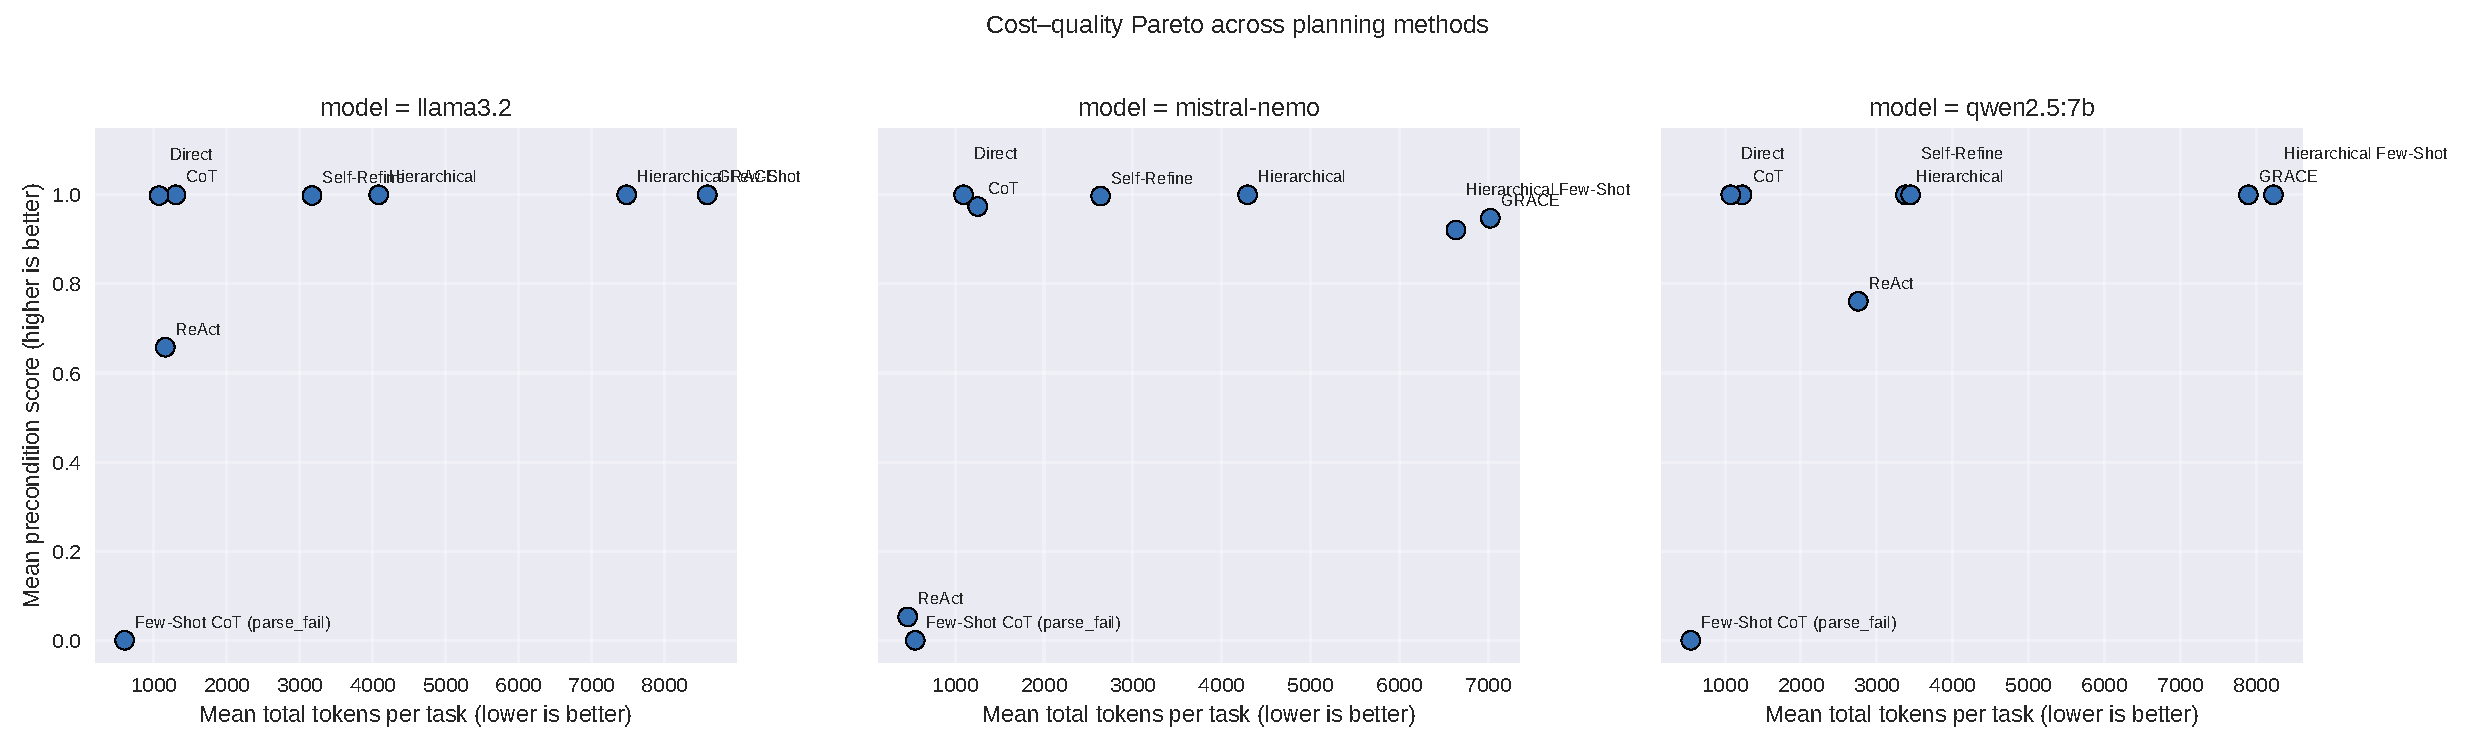
\includegraphics[width=\columnwidth]{figures/cost_quality_pareto.pdf}
  \caption{Cost--quality Pareto across planning methods and models.}
  \label{fig:pareto}
\end{figure}

\subsection{Heuristic vs strict precondition}\label{sec:strict}

A widely-reported plan-quality metric checks only that each
interaction is preceded by some \texttt{Navigate} or \texttt{Find},
without enforcing object identity, holding state, or container open
order. We re-evaluate every plan with the GRACE verifier and report
the strict score alongside the heuristic in
Figure~\ref{fig:strict}. Baselines that look perfect under the
heuristic collapse under the strict check, while GRACE retains its
score by construction.

\begin{figure}[t]
  \centering
  \includegraphics[width=\columnwidth]{figures/precondition_strict_vs_heuristic_qwen2.5_7b.pdf}
  \caption{Heuristic vs strict precondition --- \texttt{qwen2.5:7b}.}
  \label{fig:strict}
\end{figure}

\subsection{Execution table (AI2-THOR)}\label{sec:exec}

% tables/table_sim.tex not found — run:
%   python scripts/gen_latex_table.py --table sim \
%       --csv results/<run_id>/sim_qwen2.5_7b.csv \
%       --out paper/tables/table_sim.tex

\subsection{Ablation}\label{sec:ablation}

We isolate the contribution of each GRACE component by disabling it
in turn: \texttt{GRACE-NoVerifier} (no symbolic gate),
\texttt{GRACE-NoRepair} (replan falls back to global, not local), and
\texttt{GRACE-NoMemory} (no few-shot retrieval). Results are in
Figure~\ref{fig:ablation}; the full numbers are in the appendix.

\begin{figure}[t]
  \centering
  \includegraphics[width=\columnwidth]{figures/ablation_qwen2.5_7b.pdf}
  \caption{GRACE ablation on \texttt{qwen2.5:7b}.}
  \label{fig:ablation}
\end{figure}

\subsection{Failure cases}\label{sec:failure}

We hand-label GRACE failures on the 38-task set into three
categories: (i) object-naming ambiguity (a synonym the verifier
cannot match), (ii) mis-decomposition (high-level LLM omits a
required sub-goal), and (iii) sub-goal-boundary mismatch (the failed
step actually serves a future sub-goal). Object-naming ambiguity
dominates and is orthogonal to the planning strategy.

\subsection{Discussion}\label{sec:discussion}

GRACE's contribution is a \emph{deterministic} verifier and a
\emph{localised} repair operator integrated with hybrid memory. The
verifier costs zero tokens and runs in $O(|\pi|)$, yet exposes
silent precondition violations that fool the heuristic metric. The
local repair operator keeps already-completed work intact, which the
ablation shows is essential to GRACE's token economy. The hybrid
memory store grows over time, giving GRACE a smooth cold-start to
long-running-deployment path that single-source few-shot baselines
do not offer.
